%
% 公立はこだて未来大学卒業研究中間報告書[全コース対応版]
%
%         ファイル名:"sample.tex"
%
\documentclass[11pt]{ujarticle}
\usepackage{funinfosys}
\usepackage{url}
\usepackage[dvipdfmx]{graphicx}

\author{% 
1020259 中村碧\\指導教員 : 松原克弥
}
\course{Intelligent Systems Course}

\title{Wii Fit BoardとSphero SPRK+による直感的なロボット制御のためのMROS2の活用}
\etitle{}
\eauthor{Aoi Nakamura}
\abstract{今日、子供に科学技術やエンジニアリング、数学等に興味を抱くきっかけとしてロボットを活用した教育手法が発案されている。
しかし、教育環境の限られた時間やリソース、教育ニーズの変化や異なる学習スタイルに対応したソフトウェア基盤の存在は少ない。
また、ロボットの制御方法としてはプログラミングを用いたものが多く、人間とロボットの相互作用(Human-Robot-Interraction)を直感的に感じられるない場合が多い。
\\ 本研究は、mROS2を利用して体の動きに基づくゲームコントローラーであるWii Fit Boardと教育用ロボットであるSphero SPRK+が連携するためのミドルウェア層を実装し、ユーザーが物理的なジェスチャーを通じてロボットを制御することで,mROS2の拡張性を示すことを目指す。
}
\keywords{ロボティクス,mROS2,HRI(Human Robot Interraction)}
\eabstract{
\\}
\ekeywords{Roboethics, mROS2, HRI(Human Robot Interraction)}
\begin{document}
\maketitle
%\vspace*{-.5cm}

\section{背景と目的}
%目的



\section{スクレイピング}


\begin{figure}[h]
	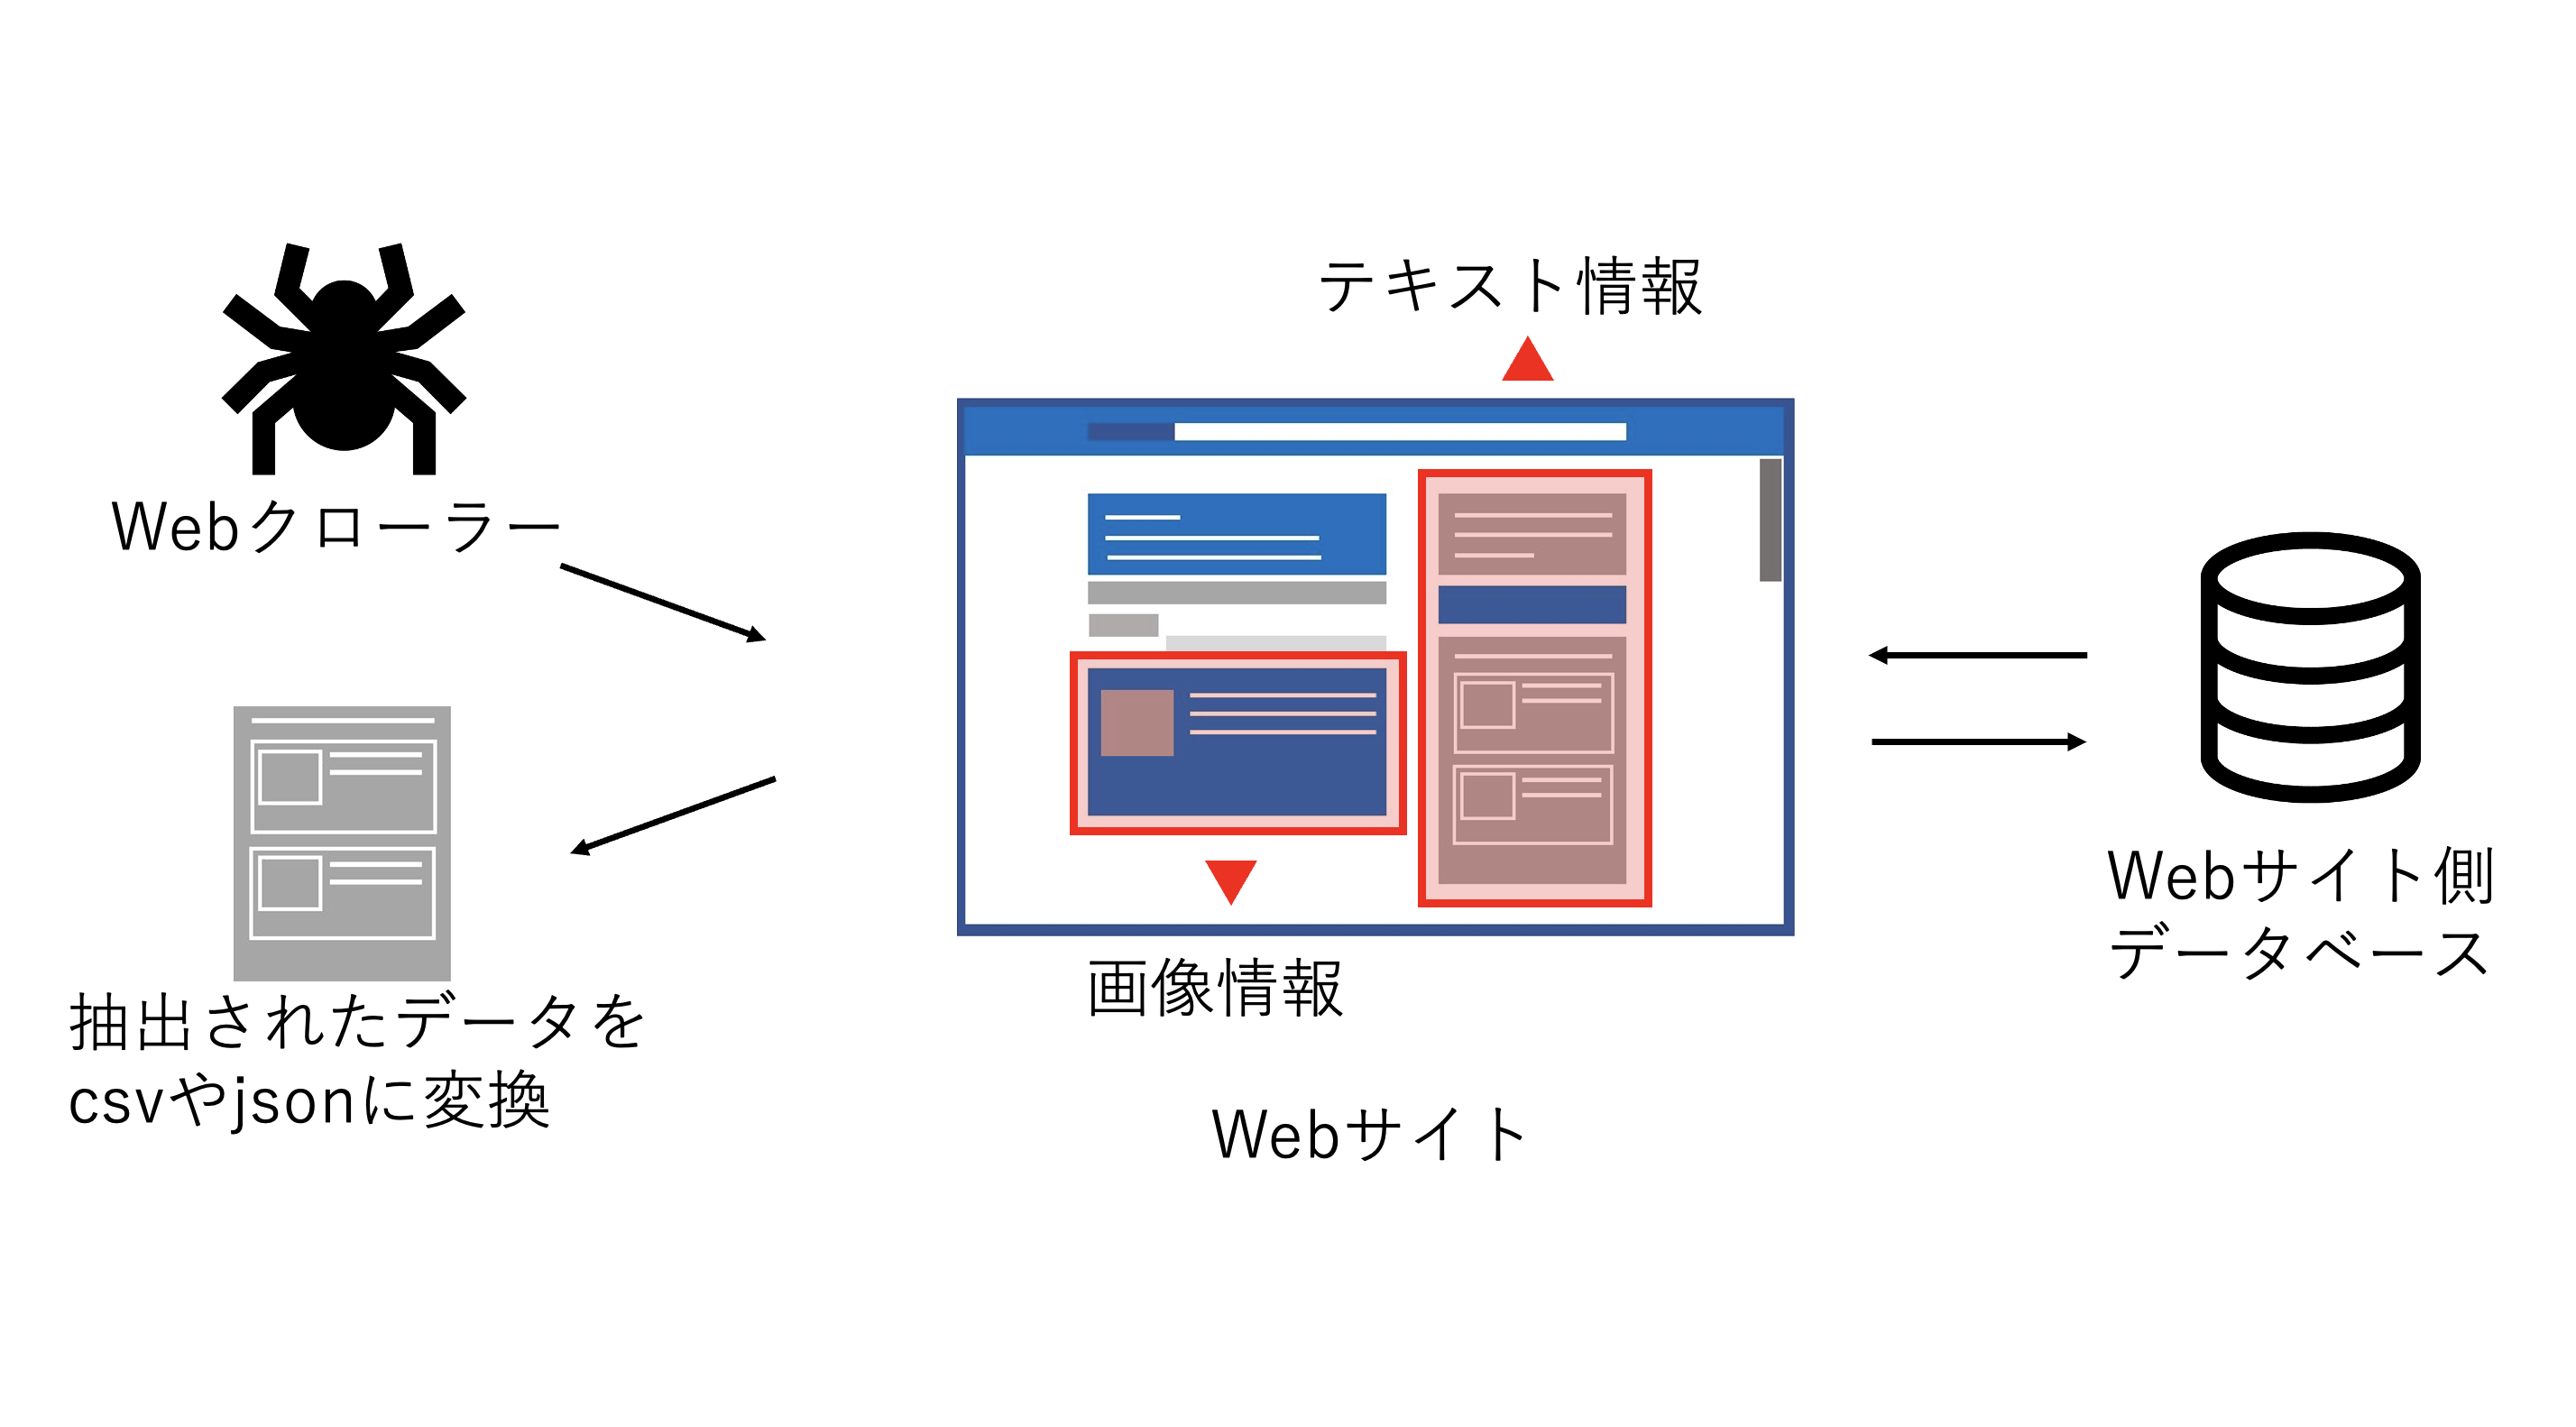
\includegraphics[width=0.9\linewidth]{./src/selenium.png}
	\caption{スクレイピングの解説}
  \label{fig:arch}
\end{figure}

\section{提案}



\section{実装}


\section{進捗と計画}


\section{まとめ}


\section{情報システムコースにおける本研究の位置づけ}


\begin{thebibliography}{99}
	\bibitem{rikkyo}
	立教大学, "立教大学シラバス検索システム", 立教大学. [Online]. Available from: \url{https://www.rep-rikkyo.com/class_rooms?day=c&hour=4}. Accessed: 2023-10-25.
	\bibitem{gakugei}
	東京学芸大学 (非公式), "東京学芸大学教室検索システム", 東京学芸大学. [Online]. Available from: \url{https://u-gakugei-uoa.pages.dev/akitan/}. Accessed: 2023-10-25.
	\bibitem{selenium}
	SeleniumHQ, "Selenium Documentation", Selenium, 2023. [Online]. Available from: \url{https://www.selenium.dev/documentation/en/}. Accessed: 2023-10-25.
\end{thebibliography}
\end{document}
%
%
% EOF 
